\documentclass[a4paper,12pt]{article}
\makeatletter
\renewcommand{\@seccntformat}[1]{}
\makeatother
%%% Работа с русским языком			% поиск в PDF
\usepackage{mathtext} 				% русские буквы в формулах
\usepackage[T2A]{fontenc}			% кодировка
\usepackage[utf8]{inputenc}			% кодировка исходного текста
\usepackage[english, russian]{babel}	% локализация и переносы
\usepackage{indentfirst}
\frenchspacing
\usepackage{lscape}
%%% Дополнительная работа с математикой
\usepackage{amsmath,amsfonts,amssymb,amsthm,mathtools} % AMS
\usepackage{icomma} % "Умная" запятая: $0,2$ --- число, $0, 2$ --- перечисление

%% Номера формул
%\mathtoolsset{showonlyrefs=true} % Показывать номера только у тех формул, на которые есть \eqref{} в тексте.
%\usepackage{leqno} % Нумерация формул слева

%% Свои команды
\DeclareMathOperator{\sgn}{\mathop{sgn}}

%% Перенос знаков в формулах (по Львовскому)
\newcommand*{\hm}[1]{#1\nobreak\discretionary{}
	{\hbox{$\mathsurround=0pt #1$}}{}}

%%% Работа с картинками
\usepackage{graphicx}  % Для вставки рисунков
\setlength\fboxsep{3pt} % Отступ рамки \fbox{} от рисунка
\setlength\fboxrule{1pt} % Толщина линий рамки \fbox{}
\usepackage{wrapfig} % Обтекание рисунков текстом

%%% Работа с таблицами
\usepackage{array,tabularx,tabulary,booktabs} % Дополнительная работа с таблицами
\usepackage{longtable}  % Длинные таблицы
\usepackage{multirow} % Слияние строк в таблице

%%% Программирование
\usepackage{etoolbox} % логические операторы

%%% Страница
\usepackage{extsizes} % Возможность сделать 14-й шрифт
\usepackage[margin=1in]{geometry} % Простой способ задавать поля
\geometry{top=20mm}
\geometry{bottom=20mm}
\geometry{left=15mm}
\geometry{right=15mm}

\usepackage{fancyhdr}

\pagestyle{fancy}
\fancyhf{}
\fancyhead[L]{\slshape\nouppercase{\leftmark}}
\cfoot{\thepage}

%\usepackage{fancyhdr} % Колонтитулы
% 	\pagestyle{fancy}
%\renewcommand{\headrulewidth}{0pt}  % Толщина линейки, отчеркивающей верхний колонтитул
% 	\lfoot{Нижний левый}
% 	\rfoot{Нижний правый}
% 	\rhead{Верхний правый}
% 	\chead{Верхний в центре}
% 	\lhead{Верхний левый}
%	\cfoot{Нижний в центре} % По умолчанию здесь номер страницы

\usepackage{setspace} % Интерлиньяж
%\onehalfspacing % Интерлиньяж 1.5
%\doublespacing % Интерлиньяж 2
%\singlespacing % Интерлиньяж 1

\usepackage{lastpage} % Узнать, сколько всего страниц в документе.

\usepackage{soul} % Модификаторы начертания

\usepackage{hyperref}
\usepackage[usenames,dvipsnames,svgnames,table,rgb]{xcolor}
\hypersetup{				% Гиперссылки
	unicode=true,           % русские буквы в раздела PDF
	pdftitle={Заголовок},   % Заголовок
	pdfauthor={Автор},      % Автор
	pdfsubject={Тема},      % Тема
	pdfcreator={Создатель}, % Создатель
	pdfproducer={Производитель}, % Производитель
	pdfkeywords={keyword1} {key2} {key3}, % Ключевые слова
	colorlinks=true,       	% false: ссылки в рамках; true: цветные ссылки
	linkcolor=blue,          % внутренние ссылки
	citecolor=blue,        % на библиографию
	filecolor=magenta,      % на файлы
	urlcolor=magenta          % на URL
}

\usepackage{csquotes} % Еще инструменты для ссылок

%\usepackage[style=authoryear,maxcitenames=2,backend=biber,sorting=nty]{biblatex}

\usepackage{multicol} % Несколько колонок

\usepackage{tikz} % Работа с графикой
\usepackage{pgfplots}
\usepackage{pgfplotstable}
%\usepackage[backend=biber, bibencoding=utf8, sorting=nty, babel=other, maxcitenames=2, bibstyle=apa, style=authoryear, sortcites, sortlocale=auto]{biblatex}
\usepackage[backend=biber, bibencoding=utf8, sorting=nty, maxcitenames=2, bibstyle=apa, style=authoryear]{biblatex}

\addbibresource{bibliography.bib}
\renewcommand*{\nameyeardelim}{\addcomma\space}

\date{\today}

\setcounter{secnumdepth}{0}

\begin{document}
	
	\begin{titlepage}
		\newpage
		
		\begin{center}
			\large{Федеральное государственное автономное образовательное учреждение высшего образования} \\
		\end{center}
		
		\begin{center}
			\large \textbf{НАЦИОНАЛЬНЫЙ ИССЛЕДОВАТЕЛЬСКИЙ УНИВЕРСИТЕТ
				«ВЫСШАЯ ШКОЛА ЭКОНОМИКИ»
			} \\
		\end{center}
		
		\vspace{1em}
		
		\begin{center}
			\Large \textbf{Факультет экономических наук} \\
		\end{center}
		\begin{center}
			\large {по направлению подготовки Экономика} \linebreak \large {образовательная программа «Экономика»}
			
		\end{center}
		
		\vspace{2em}
		
		\vspace{0.5em}
		\rule{\linewidth}{0.3mm}
		\begin{center}
			\huge \textbf{Домашняя работа №1} \\[0.4cm]
			\LARGE \textbf{В рамках курса
				«Микроэконометрика качественных данных»
}
		\end{center}
		\rule{\linewidth}{0.3mm} \\[0.4cm]
		
		\vspace{18em}
		\begin{flushright}
			\large
			\textit{Выполнил:}\\
			Максим \textsc{Пешков} \\
			\textit{Группа:}\\
			БЭК181
			% Your name
		\end{flushright}
		
		\vspace{5em}
		
		\begin{center}
			Москва, 2021
		\end{center}
		
	\end{titlepage}
	
	\newpage
	
	\tableofcontents
	
	\listoftables
	
	
	\section{О данных}
	
	В данной работе мы будем изучать, как различные факторы влияют на вероятность
	того, что индивид оформит подписку на онлайн кинотеатр.
	
	Данные содержат информацию о следующих индивидуальных характеристиках:
	\begin{itemize}
		
		\item income — доход
		
		\item age — возраст
		
		\item internet — доля свободного времени, проводимого в интернете
		
		\item series — количество просмотренных за год сериалов
		
		\item health — субъективная оценка здоровья
		
		\item male — половая принадлежность (1 – мужчина, 0 – женщина)
		
		\item marriage — состоит в официальном браке
		
		\item residence — место проживания
		
		\item cat — факт наличия кота
		
		\item news — субъективная оценка степени, в которой индивид интересуется новостями
		
		\item sub — факт наличия подписки на онлайн кинотеатр (\textbf{зависимая переменная})
		
		\item TV — индивид смотрит телевизор не реже раза в неделю.
		
	\end{itemize}
	 
\newpage	

	\section{Часть 1. Теория и гипотезы}
	
	\subsection{Задание №1.1.}
	\textit{
			Выберите независимые переменные. Кратко теоретически обоснуйте выбор каждой из них: не обязательно со ссылками на литературу, достаточно здравого смысла. Укажите и кратко обоснуйте предполагаемые направления эффектов. При этом вам понадобится как минимум одна непрерывная переменная (например, возраст или доход) и одна дамми переменная (например, половая принадлежность или брак). Не рекомендуется брать больше трех различных независимых переменных, не считая их нелинейных преобразований: квадрат, логарифм, перемножение с целью получения переменной взаимодействия и т. д.
	}
	
	\vspace{0.2cm}
	
	В качестве независимых переменных будут использоваться переменные \textbf{internet, TV, age, series}.
	
	\begin{itemize}
		\item \textbf{series}
		
		На выбор покупки онлайн подписки влияет заинтересованность человека в просмотре сериалов в целом. И чем больше индивид смотрит сериалов, тем больше вероятность, что он использует онлайн кинотеатр, а если он их смотрит мало, то такие издержки за оплату подписки ему будут невыгодны и он не будет использовать онлайн кинотеатр вовсе. Поэтому ожидается наблюдение положительного эффекта.
		
		
		\item \textbf{internet}
		
		Чем чаще люди проводят время в интернете, тем более осведомлены о подписках в онлайн-кинотеатрах, а также им может казаться проще и выгоднее оформить подписку, так как на сегодняшний день большая часть онлайн кинотеатров существуют в одной экосистеме с другими сервисами (например, Кинопоиск и Яндекс). Поэтому ожидается наблюдение положительного эффекта.
		
		\item \textbf{TV}
		
		Такие способы просмотра сериалов или кино как телевидение и онлайн-кинотеатры могут быть взаимозаменяемыми для некоторых людей, поэтому выбор одного может исключать выбор другого, так как при покупке подписки уже не будет смысла в телевидении (на платформе онлайн-кинотеатра часто есть те же самые фильмы или вовсе уникальные), а при частом просмотре телевидения может быть невыгодно переходить на онлайн-кинотеатр, так как интересные для индивида фильмы показывают по телевидению. Поэтому ожидается наблюдение отрицательного эффекта.
		
		\item \textbf{age}
		
		Выбор этой переменной обоснован тем, что заинтересованность в онлайн-кинотеатрах различна среди поколений. Старшее поколение и более взрослые люди воспринимают это как новинку и не видят в нем необходимость, так как часто используют телевидение для просмотра фильмов или сериалов. А молодое поколение наоборот, чаще использует интернет и онлайн-просмотр для фильмов. Поэтому ожидается наблюдение положительного эффекта.
	\end{itemize}

	\vspace{1cm}

	\subsection{Задание №1.2.}
		\textit{
				Сформулируйте по крайней мере одну гипотезу о наличии эффекта взаимодействия и нелинейного эффекта (например, квадратичного). Теоретически обоснуйте выдвигаемые вами гипотезы. Включите соответствующие переменные в вашу модель. При этом переменная, входящая нелинейно, должна иметь и линейную часть.
	}

		 \vspace{0.2cm}
		 
	Будут проверяться две нелинейные гипотезы: о наличии эффекта взаимодействия переменных \textbf{internet, TV}; о наличии квадратичного эффекта \textbf{age}. Ниже приведены обоснования для этого.
	
	\begin{itemize}
		\item \textbf{Эффекта взаимодействия переменных \textbf{internet, TV}}
		
		Использование интернета по-разному влияет на выбор подписки у людей, которые часто смотрят телевидение и нет. Чем чаще индивид смотрит телевидение, тем для его выбора частое использование интернета менее важно, так как, скорей всего, он просматривает интересующие его фильмы или сериалы по ТВ и у него нет заинтересованности в оформлении подписки на онлайн кинотеатр. А при не частом просмотре телевидения большое количество времени в интернете может как раз и означать, что он тратит его часть на просмотры чего-либо в онлайн кинотеатре. Тем самым, ожидается наблюдение отрицательного эффекта у интеракции между переменными - отрицательный эффект взаимодействия.

		\item \textbf{Квадратичная зависимость от age}
		
		Оплата подписки в онлайн кинотеатре может казаться высокой для людей с низким уровнем дохода, которыми чаще всего являются молодые люди или пенсионеры. Более того, у молодых людей может не хватать свободного времени на просмотры фильмов или сериалов в любом формате из-за других интересов в свободное время: активная учеба, занятия спортом или прогулки и общения с друзьями. А для более старого поколения использование онлайн-кинотеатров может быть сложным и труднодоступным. Поэтому ожидается наблюдение перевернутого U-образного эффекта от возраста, то есть перед линейной компонентой будет положительный знак, а перед квадратичной - отрицательный (отрицательный эффект для молодых и пожилых людей).
		
	\end{itemize}
	
	\newpage
	
	\section{Часть 2. Линейно-вероятностная модель.}
	
	\subsection{Задание №2.1.}
		\textit{
				 Оцените линейно-вероятностную модель, предварительно записав регрессионное уравнение. Укажите оцениваемые параметры и метод получения оценок. Результат представьте в форме таблицы (можно, например, использовать выдачу из stata, R или python).
		}

	 \vspace{0.2cm}
	
	Для проверки выше перечисленных гипотез в линейно-вероятностной модели будет использоваться следующее регрессионное уравнение:
	
	\begin{align*}
		sub_i = \beta_0+\beta_1 \times series_i+ \beta_2 \times internet _i+ \beta_3 \times TV_i + \beta_4 \times age_i + \beta_5 \times age_i^2 +\beta_6 \times internet_i \times TV_i + \varepsilon_i
	\end{align*}
	
	Для нахождения оцениваемых параметров $\beta_i$ в линейно-вероятностной модели используется метод наименьших квадратов (МНК), то есть параметры оцениваются и находятся аналитически по такой формуле $\hat\beta = (X^TX)^{-1}X^T$. Результаты найденных оценок представлены ниже в Таблице \ref{linear}.
	
	\begin{table}[!h] \centering 
		  \caption{Результаты линейно-вероятностной модели} 
		  \label{linear} 
		  \small
		\begin{tabular}{@{\extracolsep{5pt}}lc} 
		\\[-1.8ex]\hline 
		\hline \\[-1.8ex] 
		 & \multicolumn{1}{c}{\textit{Dependent variable:}} \\ 
		\cline{2-2} 
		\\[-1.8ex] & sub \\ 
		\hline \\[-1.8ex] 
		 series & 0.026$^{***}$ \\ 
		  & (0.002) \\ 
		  & \\ 
		 internet & 0.248$^{***}$ \\ 
		  & (0.044) \\ 
		  & \\ 
		 TV & $-$0.227$^{***}$ \\ 
		  & (0.030) \\ 
		  & \\ 
		 age & 0.005$^{***}$ \\ 
		  & (0.002) \\ 
		  & \\ 
		 $age^2$ & $-$0.00002$^{*}$ \\ 
		  & (0.00001) \\ 
		  & \\ 
		 internet$\times$TV & $-$0.045 \\ 
		  & (0.054) \\ 
		  & \\ 
		 Constant & 0.096$^{*}$ \\ 
		  & (0.052) \\ 
		  & \\ 
		\hline \\[-3ex] 
		Observations & 5,000 \\ 
		R$^{2}$ & 0.090 \\ 
		Adjusted R$^{2}$ & 0.089 \\ 
		F Statistic & 82.296$^{***}$ (df = 6; 4993) \\ 
		AIC            & $6365.68$     \\
		BIC            & $6417.82$     \\
		\hline 
		\hline \\[-1.8ex] 
		\textit{Note:}  & \multicolumn{1}{r}{$^{*}$p$<$0.1; $^{**}$p$<$0.05; $^{***}$p$<$0.01} \\ 
	\end{tabular} 
	\end{table} 
			
	\subsection{Задание №2.2.}
	
	\textit{
			Перечислите основные недостатки линейно-вероятностной модели. Напишите, можно ли интерпретировать оценки коэффициентов, их значимость (с использованием обычной оценки ковариационной матрицы), коэффициент детерминации и F-статистику?
			Если да, то приведите интерпретацию, а если нет, то объясните (без непосредственной реализации), почему она в данном случае невозможна и предложите альтернативный способ оценки качества модели.
	}
	
	
	\vspace{0.2cm}
	
	Недостатки линейно-вероятностной модели заключаются в следующем:
	
	\begin{itemize}
		\item Гетероскедастичность
		
		Из-за того, что $Var(\varepsilon_i) = x_i'\beta(1-x_i'\beta)$, то есть для каждого наблюдения ошибка зависит от зависимых переменных, то в этой модели есть гетероскедастичность. Следствием чего является неэффективность оценок.
		
		\item Ненормальность распределения ошибок
		
		В этой модели ошибки распределены следующим образом:
		
		\begin{equation*}
			\begin{cases}
				\varepsilon_i = 1-x_i'\beta \text{, если $y_i=1$}\\
				\varepsilon_i = -x_i'\beta \text{, если $y_i=0$}
			\end{cases}
		\end{equation*}
	
		Это ведет к тому, что не следует проверять гипотезы и интерпретировать полученные $R^2$ и $F$-статистику при малом количество наблюдений.
				
		\item Неинтерпретируемость оценок коэффициентов
		
		Через оценки данной модели выражается вероятность $\hat{p_i}=x_i'\hat{\beta}$, которая может не лежать на интервале $[0, 1]$, так как при оценки МНК нет ограничения на вхождение в этот интервал, из-за чего невозможно правильно интерпретировать оценки коэффициентов.
		
	\end{itemize}
	
	Предложения для оценки качества модели и проверки гипотез:
	
	\begin{itemize}
		\item  Для борьбы с гетероскедастичностью можно использовать Обобщенный МНК с ковариационной матрицей устойчивой к гетероскедастичности
		
		\item Для оценивания качества модели можно использовать AIC, BIC или качество точности модели - $accuracy$
		
		\item Для оценивания гипотез о значимости коэффициентов можно использовать бутстрапированные доверительные интервалы и проверять будет ли лежать 0 в данном ассимптотическом доверительном интервале
		
	\end{itemize}
	
	
	\subsection{Задание №2.3.}
	
	\textit{
			Оцените и проинтерпретируйте, независимо от значимости, предельные эффекты на вероятность подписки каждой из используемых вами независимых переменных, предварительно записав формулы, по которым осуществлялся расчет. Результат представьте в форме таблицы, где для переменных, входящих нелинейно, рассчитан средний предельный эффект. Также, для этих переменных должно быть указано, при каких значениях независимой переменной их предельный эффект является положительным, а при каких — отрицательным.
	}
	
	\vspace{1cm}
	
	Формулы для оценивания предельных эффектов в этой модели:
	
	\begin{align*}
		\dfrac{\partial sub_i}{\partial series_i} &= \hat{\beta_1}\\
		\dfrac{\partial sub_i}{\partial internet_i} &= \hat{\beta_2}+\hat{\beta_6}*TV_i\\
		\dfrac{\partial sub_i}{\partial age_i} &= \hat{\beta_5}+ 2*\hat{\beta_6}*age_i\\
		sub_i |_{TV_i=1} - sub_i |_{TV_i=0} &= \beta_3 + \beta_6 *internet_i
	\end{align*}
	
	Средний предельный эффект может оцениваться 2 способами: среднее всех предельных эффектов в точках (AME), предельный эффект в точке со средними показателями (MME). Так как в условиях не сказано какой из них считать, то будем расчитать MME.
	
	Ниже представлена Таблица \ref{MElinear} с найденными средними предельными эффектами для переменных  $age, internet, TV$, а также предельный эффект для $series$, записанные в колонке MME. Также для переменных входящих нелинейно записано когда предельный эффект принимает отрицательные значения, а когда положительные.
	
	\begin{table}[h]
		\caption{Средние предельные эффекты для линейно-вероятностной модели}
		\label{MElinear}
		\centering
		\begin{tabular}{|c|c|c|c|c|c|}
			\hline
			переменная &  MME  & отрицательные& положительные&min&max\\ 
			\hline
			series &0.0262 &-&-&0.0262&0.0262\\ 
			\hline
			internet  &0.2190 &-& $\forall$ TV&0.212&0.2475\\ 
			\hline
			TV &-0.2472&при любых значениях internet& - &-0.2677&-0.2272 \\ 			
			\hline
			age  &0.0017 &[95.68114, +$\inf$) &[0, 95.68114)&-0.0002 &0.0036\\ 
			\hline
		\end{tabular}
	\end{table}

	Как видно из таблицы предельные эффекты для $internet, series$ положительные, что говорит о положительном направлении эффектов от количества просмотренных сериалов и времени в интернете на оформление подписки онлайн-кинотеатра. Средний предельный эффект от количества времени в интернете говорит о том, что при увеличении доли свободного времени в интернете на 10\% (0.1) вероятность оформления подписки вырастет на 21.9\% при прочих равных, а вот увеличение просмотренных сериалов на 1 увеличивает вероятность оформления подписки на 26.2\% при прочих равных. 
	
	Однако разница в частоте просмотра телевидения дает негативный предельный эффект, как и ожидалось, то есть при увеличении частоты просмотра ТВ и изменения переменной с 0 до 1 вероятность уменьшается на 24.72\%. 
	
	Для возраста предельный эффект разный в зависимости от возраста. Для людей младше 95 лет предельный эффект положительный, а для людей старше отрицательный.


	\newpage
	
	\section{Часть 3. Пробит модель.}

	\subsection{Задание №3.1.}
	\textit{
		Оцените пробит модель, предварительно записав максимизируемую функцию правдоподобия, указав оцениваемые параметры и метод получения оценок, а также их основные свойства. Результат представьте в форме таблицы (можно, например, использовать выдачу из stata, R или python). }

	
	\vspace{0.2cm}
	
	Для оценивания пробит модели применяется метод максимального правдоподобия, где максимизируемая функцию правдоподобия равна
	
	\begin{align*}
		\L = \prod_{i=1}^{n}\left(\mathcal{F} (x_i'\beta)\right)^{sub_i} \left(1-\mathcal{F} (x_i'\beta)\right)^{1-sub_i} \rightarrow max_{\beta_i}
	\end{align*}
	
	 Где $x_i$ - вектор  $(series_i, internet_i, TV_i, age_i, age_i^2, internet_i\times TV_i)$, $\beta$ - тоже вектор оцениваемых параметров $\beta_i, i = \overline{0, 6}$, $\mathcal{F} = \frac{1}{\sqrt{2\pi}}\int_{-\inf}^z e^{\frac{t^2}{2}}dt$ - функция стандартного нормального распределения. 

	\vspace{0.2cm}
	
	Результаты найденных оценок представлены в Таблице \ref{probit}.
	
	\begin{table}[!h] \centering 
	  \caption{Результаты пробит модели} 
	  \label{probit} 
	  \small
	\begin{tabular}{@{\extracolsep{5pt}}lc} 
	\\[-1.8ex]\hline 
	\hline \\[-1.8ex] 
	 & \multicolumn{1}{c}{\textit{Dependent variable:}} \\ 
	\cline{2-2} 
	\\[-1.8ex] & sub \\ 
	\hline \\[-1.8ex] 
	 series & 0.077$^{***}$ \\ 
	  & (0.007) \\ 
	  & \\ 
	 internet & 0.632$^{***}$ \\ 
	  & (0.123) \\ 
	  & \\ 
	 TV & $-$0.693$^{***}$ \\ 
	  & (0.087) \\ 
	  & \\ 
	 age & 0.013$^{***}$ \\ 
	  & (0.005) \\ 
	  & \\ 
	 $age^2$ & $-$0.0001$^{*}$ \\ 
	  & (0.00004) \\ 
	  & \\ 
	 internet$\times$TV & $-$0.007 \\ 
	  & (0.154) \\ 
	  & \\ 
	 Constant & $-$1.135$^{***}$ \\ 
	  & (0.151) \\ 
	  & \\ 
	\hline \\[-1.8ex] 
	Observations & 5,000 \\ 
	Log Likelihood & $-$3,021.975 \\ 
	Akaike Inf. Crit. & 6,057.949 \\ 
	\hline 
	\hline \\[-1.8ex] 
	\textit{Note:}  & \multicolumn{1}{r}{$^{*}$p$<$0.1; $^{**}$p$<$0.05; $^{***}$p$<$0.01} \\ 
	\end{tabular} 
	\end{table} 

\vspace{0.2cm}
	Основные свойства оценок пробит модели, полученных методом максимизации правдоподобия, заключаются в 
	
	\begin{itemize}
		\item Состоятельны
		\item Асимптотически несмещенные
		\item Асимптотически нормальны
		\item Асимптотически эффективны
		\item Инвариантны
	\end{itemize}

		
	\subsection{Задание №3.2.}
	\textit{
	Проинтерпретируйте оценки коэффициентов для каждой независимой переменной. Поясните, как полученные результаты соотносятся с высказанными вами ранее предположениями. }

	\vspace{0.2cm}
	
	Для пробит модели само значение коэффициента нельзя никак численно интерпретировать, можно только его знак для некоторых переменных, что и будет сделано ниже.
	
	\begin{itemize}
			\item	Для переменной $series$ коэффициент положительно значим для вероятности оформления подписки онлайн кинотеатра. Такой же положительный эффект для количества просмотренных сериалов предполагался выше.
			\item 	Частота просмотра телевидения $TV$ отрицательно и значимо влияет на вероятность оформления подписки онлайн кинотеатра, что соотносится с высказанными предположениями
			\item 	Доля времени в интернете $internet$ положительно и значимо влияет на вероятность оформление подписки онлайн кинотеатра, что соотносится с высказанными предположениями
			\item 	Возраст $age$ влияет на вероятность наличия подписки онлайн кинотеатра перевернутой U-образной зависимостью, как и ожидалось в выказанных предположениях. Хотя и коэффициент перед линейной переменной значим на любом адекватном уровне значимости, а перед квадратом только на 10 \% значимости.
			\item По оцененным параметрам можно сказать, что не наблюдается значимости перед выбранным эффектом взаимодействия, причем ожидалась отрицательная значимость. Хотя оценка коэффициента перед интеракцией доли времени в интернете и частотой просмотра телевидения имеет отрицательный знак, что соответствует о предположении направления эффекта.
	\end{itemize}
	
	\subsection{Задание №3.3.}
	\textit{
	Оцените вероятность наличия подписки для индивида с произвольными (например, вашими) характеристиками. Запишите формулу, по которой осуществлялся расчет (подставьте в нее полученные реализации оценок). }
	
	\vspace{1cm}
	
	Оценим вероятность наличия подписки для индивида с такими характеристиками, представленные в Таблице \ref{individ1}.
	
	\begin{table}[!h]
		\caption{Характеристики рассматриваемого индивида}
		\label{individ1}
		\centering
		\small
		\begin{tabular}{|c|c|}
			\hline
			Переменная &  Значение  \\ 
			\hline
			$series_{ind} $ &4 \\ 
			\hline
			$internet_{ind} $ &0.7 \\ 		
			\hline
			$TV_{ind} $ &0 \\ 	
			\hline
			$age_{ind} $ &21 \\ 
			\hline
		\end{tabular}
	\end{table}

	\vspace{1.5cm}

	Вероятность наличия подписки для индивида оценивается по следующей формуле:
	
	\begin{align*}
		P(sub_{ind}=1)= \mathcal{F} (\hat{\beta_0} + \hat{\beta_1} \times series_{ind}+ \hat{\beta_2} \times internet _{ind} +\hat{\beta_3}  \times TV_{ind} \\+ \hat{\beta_4} \times age_{ind} + \hat{\beta_5}\times age_{ind}^2 +\hat{\beta_6} \times internet_{ind} \times TV_{ind}) 
	\end{align*}

	Где $\hat{\beta_i}$ - оцененные параметры в модели, вместо регрессоров подставляются их соответствующие значения, а $\mathcal{F} = \frac{1}{\sqrt{2\pi}}\int_{-\inf}^z e^{\frac{t^2}{2}}dt$ - функция стандартного нормального распределения. 
	
	\begin{align*}
		P(sub_{ind}=1)= \mathcal{F} (-1.135+0.077\times series_{ind}+ 0.632 \times internet _{ind} -0.693 \times TV_{ind} \\+ 0.013\times age_{ind} - 0.0001\times age_{ind}^2-0.007  \times internet_{ind} \times TV_{ind}) \\
		P(sub_{ind}=1)= \mathcal{F} (-1.135+0.077\times 4 + 0.632 \times 0.7 -0.693 \times 0 + 0.013\times 21- 0.0001\times 21^2\\-0.007  \times 0.7 \times 0)
	\end{align*}
	
	Найденное значение равно 0.4464257, то есть с вероятностью в 44.64\% у рассмотренного индивида есть подписка на онлайн кинотеатр.
	
	\subsection{Задание №3.4.}
	\textit{
	Для произвольных непрерывной и бинарной независимых переменных оцените средний предельный эффект на вероятность наличия подписки, предварительно записав формулы (с подставленными реализациями оценок), по которым осуществлялся расчет. Результат представьте в форме таблицы. }
	
	\vspace{0.4cm}
	
	Оценим средние предельные эффекты для непрерывной переменной $age$ и бинарной переменной $TV$. Формулы для нахождения их среднего предельнего эффекты (MME):
	
	\begin{itemize}
		\item для непрерывной переменной $age$ средний предельный эффект считается как
		
			\begin{align*}
				\dfrac{\partial P(sub=1)}{\partial age} = f (\overline{x}'\hat{\beta})\times (\hat{\beta_4} +
				2*\hat{\beta_6}*\overline{age})
			\end{align*}
		
			Где $\overline{x}$ - средние значения регрессоров модели, $\overline{age}$ - среднее значение возраста в выборке, а $f=\frac{1}{\sqrt{2\pi}} e^{\frac{t^2}{2}}$ - функция плотности стандартного нормального распределения.
			
		
		\item для бинарной переменной $TV$ средний предельный эффект считается как разница
		
		\begin{align*}
			\Delta P(sub=1) = P(sub=1|\overline{x_{-TV}},TV=1)-P(sub=1|\overline{x_{-TV}},TV=0) = \\
			= \mathcal{F} (\hat{\beta_0} + \hat{\beta_1} \times \overline{series}+ \hat{\beta_2} \times \overline{internet} +\hat{\beta_3}  \times 1 + \hat{\beta_4} \times \overline{age} + \hat{\beta_5}\times \overline{age}^2 +\hat{\beta_6} \times \overline{internet}\times 1) - \\
			- \mathcal{F} (\hat{\beta_0} + \hat{\beta_1} \times \overline{series}+ \hat{\beta_2} \times \overline{internet} +\hat{\beta_3}  \times 0 + \hat{\beta_4} \times \overline{age} + \hat{\beta_5}\times \overline{age}^2 +\hat{\beta_6} \times \overline{internet}\times 0)
		\end{align*}
	
		Где $\overline{x_{-TV}}$ - средние значения регрессоров модели кроме бинарной переменной TV, а $f=\frac{1}{\sqrt{2\pi}} e^{\frac{t^2}{2}}$ - функция плотности стандартного нормального распределения
		
	\end{itemize}

	Результаты расчета средних предельных эффектов представлены в Таблице \ref{MEprobit}.
	
	
	\begin{table}[h]
		\caption{Средние предельные эффекты для пробит модели}
		\label{MEprobit}
		\centering
		\begin{tabular}{|c|c|}
			\hline
			Переменная &  MME  \\ 
			\hline
			age  &0.001829614 \\ 
			\hline
			TV &-0.2631863 \\ 			
			\hline
		\end{tabular}
	\end{table}
	
	\subsection{Задание №3.5.}
	\textit{
	Посчитайте долю верных предсказаний и сопоставьте её с результатом наивного прогноза и линейно-вероятностной модели. Сделайте вывод о предсказательной силе пробит модели.}
	
	\vspace{0.2cm}
	
	Посчитав доли верных предсказаний, представленных в Таблице \ref{accurmodels}, можно сказать, что предсказательная сила пробит модели лучше наивной модели, но хуже чем у линейной-вероятностной модели. Тем самым, можно заключить, что пробит модель хотя и позволяет получить интерпретируемые результаты, но имеет не самую лучшую предсказательную силу.
	
	\begin{table}[!h]
		\caption{Доли верных предсказаний пробит, линейной-вероятностной, наивной модели}
		\label{accurmodels}
		\centering
		\begin{tabular}{|c|c|}
			\hline
			Модель  &  Доля верных предсказаний  \\ 
			\hline
				Пробит модель& 0.6760\\
				\hline
				Наивная модель & 0.6446\\
				\hline
				Линейно-вероятностная модель &0.6774	\\		
			\hline
		\end{tabular}
	\end{table}
	
	\subsection{Задание №3.6.}
	\textit{
	На уровне значимости 5\% проверьте гипотезу о том, что предельный эффект на вероятность наличия подписки по произвольной (на ваш выбор) независимой переменной является значимым для индивида с произвольными характеристиками. }
	
	\vspace{0.2cm}
	
	Проверим гипотезу о том, что предельный эффект на вероятность наличия подписки по переменной $series$ является значимым для индивида с произвольными характеристиками, при этом зная формулу для предельного эффекта $series$ запишем нулевую и альтернативную гипотезы.
	
	\begin{equation*}
		\begin{cases}
			H_0: \dfrac{\partial P(sub_i=1)}{\partial series_i}=f(x'\hat{\beta})\times\hat{\beta_1} = 0\\[0.3cm]
			H_a: \dfrac{\partial P(sub_i=1)}{\partial series_i}=f(x'\hat{\beta})\times\hat{\beta_1} \ne 0
		\end{cases}
	\end{equation*}
	
	Для проверки этой гипотезы необходимо использовать дельта-метод (чтобы найти дисперсию предельного эффекта), после которого тестовая статистика имеет z-распределение, так как распределение тестовой статистики будет асимптотически нормальным.
	
	Так как в условии задания не написано, что необходимо проверить гипотезу "руками", то воспользуемся пакетом \textit{margins}, которые не только считает средние предельные эффекты, но и считает z-статистику и p-value для проверки гипотезы о значимости предельного эффекта.
	
	Используя пакет \textit{margins}, легко получить, что z -статистика равна 5.8802, p-value=0.000, то есть нулевая гипотеза отвергается и предельный эффект $series$ является значимым для индивида с произвольными характеристиками.
	
	\subsection{Задание №3.7*.}
	\textit{
	Повторите предыдущий пункт для переменной, имеющей взаимодействие.}
	
	\vspace{0.2cm}
	
	Проверим гипотезу о том, что предельный эффект на вероятность наличия подписки по переменной $internet$ является значимым для индивида с произвольными характеристиками, при этом зная формулу для предельного эффекта $internet$ запишем нулевую и альтернативную гипотезы.
	
	\begin{equation*}
		\begin{cases}
			H_0: \dfrac{\partial P(sub_i=1)}{\partial internet_i}=f(x'\hat{\beta})\times(\hat{\beta_2}+\hat{\beta_7}\times TV) = 0\\[0.3cm]
			H_a: \dfrac{\partial P(sub_i=1)}{\partial internet_i}=f(x'\hat{\beta})\times(\hat{\beta_2}+\hat{\beta_7}\times TV) \ne 0
		\end{cases}
	\end{equation*}
	
	Для проверки этой гипотезы необходимо использовать дельта-метод (чтобы найти дисперсию предельного эффекта), после которого получится z-статистика, так как распределение тестовой статистики будет асимптотически нормальным.
	
	Так как в условии задания не написано, что необходимо проверить гипотезу "руками", то воспользуемся пакетом \textit{margins}, которые не только считает средние предельные эффекты, но и считает z-статистику и p-value для проверки гипотезы о значимости предельного эффекта.
	
	Используя пакет \textit{margins}, легко получить, что z -статистика равна 8.5805, p-value=0.000, то есть нулевая гипотеза отвергается и предельный эффект $internet$ является значимым для индивида с произвольными характеристиками.
	
	\section{Часть 4. Тестирование корректности спецификации пробит модели.}
	
	\subsection{Задание №4.1.}
	\textit{
	При помощи LM-теста проверьте гипотезу о соблюдении допущения о нормальном распределении случайных ошибок в пробит модели. Укажите, к каким негативным последствиям может привести нарушение данного допущения. }
	
	\vspace{0.2cm}
	
	Нарушение допущения о нормальности распределения ошибок может привести к таким негативным последствиям как
	
	\begin{itemize}
		\item Несостоятельность оценок 
		\item Возможные искажения при оценивание значимости коэффициентов
		\item Неверность проводимых тестов на значимость
	\end{itemize}
	
	Для проверки нормальности распределения ошибок воспользуемся LM тестом с использованием регрессии на единичный вектор. А именно благодаря найденным обобщенным остаткам находим градиенты по оцениваемых параметров и, регрессируя единичный вектор на них, находим $R^2$. Тогда статистика для LM теста $R^2*n$ также будет совпадать с методом через аналитические функции и будет иметь такую же хи квадрат статистику с $2$ степенями свободами.
	
	В этом тесте нулевая гипотеза будет заключаться в наличие нормального распределения ошибок, а альтернативная в отсутствии нормального распределения.
	
	\begin{equation*}
		\begin{cases}
			H_0: \varepsilon_i \sim \mathcal{N} (0, \sigma)\\
			H_a: \varepsilon_i \nsim \mathcal{N} (0, \sigma)
		\end{cases}
	\end{equation*}
	
	Проведя LM тест, получили статистику равную 0.105, а p-value равную 0.9485. То есть нулевая гипотеза не отвергается, то есть после построения регрессии наблюдается нормальность распределения ошибок, что в целом было ожидаемо, так как в выборке достаточно большое количество наблюдений (5000), а при большом количестве наблюдений по ЦПТ распределение стремится к нормальному.
	
	\subsection{Задание №4.2.}
	\textit{
	Предположите, какие переменные могут влиять на дисперсию случайной ошибки. При этом по крайней мере одна переменная должна входить и в линейный индекс основного уравнения, и в линейный индекс уравнения дисперсии. При помощи LR теста проверьте гипотезу о гомоскедастичности случайных ошибок. Запишите, к каким негативным последствиям может привести нарушение данного допущения. Объясните преимущество LM теста над LR тестом в данном случае. }
	
	\vspace{0.2cm}
	
	Как мы видели в результатах пробит модели в таблице \ref{probit}, то коэффициент перед интеракцией не значим, хотя мы предполагали значимость, что может быть вызвано гетероскедастичностью. Будем предполагать, что на дисперсию случайной ошибки влияют такие переменные, как $series, income$, так как
	
	\begin{itemize}
		\item$series$ входит в линейный индекс основного уравнения
		
		Влияние количества сериалов может влиять на дисперсию ошибки, ведь при просмотре до 3 сериалов может быть такое же безразличие и незаинтересованность в оформлении подписки на онлайн кинотеатр, а при просмотре 9 и больше сериалов появляется "сериальная" зависимость и соотношение эффектов на вероятности оформления подписки будет больше. Поэтому предполагается, что возможно наличие гетероскедастичности с зависимостью от $series$.
		
		\item $income$ входит в линейный индекс дисперсии случайной ошибки
		
		Влияние дохода очевидно при оформлении подписки, ведь не каждый человек может позволить себе тратить ежемесячно 200-300 рублей, например, достаточно бедные люди не будут заинтересованы в этом. Поэтому ошибки могут коррелировать с уровнем дохода, что ведет к гетероскедастичности.
	\end{itemize}

	Гетероскедастичность и нарушение допущения о гомоскедастичности может привести к таким негативным последствиям как:
	\begin{itemize}
		\item Неэффективность оценок
		\item Нарушение предположений ТГМ могут вести и к неправильной инерпретации значимости коэффициентов
		\item Возможно искажение в качестве модели и уменьшения предсказательной силы
	\end{itemize}

	Для проверки наличия гетероскедастичности воспользуемся LR тестом. Нулевая гипотеза заключается в наличии гомоскедастичности ошибок, а альтернативная в гетероскедастичности. 
		\begin{equation*}
		\begin{cases}
			H_0: \varepsilon_i \sim \mathcal{N} (0, \sigma)\\
			H_a: \varepsilon_i \sim \mathcal{N} (0, \sigma_i)
		\end{cases}
	\end{equation*}
	А если более точнее, то альтернативная гипотеза предполагает, что дисперсия зависима от $series, income$ как $\sigma_i=\exp(series_i* \tau_{1i}+ income_i* \tau_{2i})$, а при нулевой предполагаем, что все $\tau$ равны 0.
	
	\begin{equation*}
		\begin{cases}
			H_0: \tau = 0\\
			H_a: \text{хотя бы один из $\tau$ не равен 0}
		\end{cases}
	\end{equation*}

	Тестовая статистика равна 56.438 и имеет хи квадрат распределение c 2 степенями свободы, а p-value равен 5.554e-13, то есть нулевая гипотеза отвергается на любом разумном уровне значимости. Откуда следует, что ошибки модели гетероскедастичны.
	
	Однако выводы могут быть не совсем корректны,так как LR тест использует явный вид функции h для линейного индекса дисперсии, хотя при помощи LM теста нет необходимости предполагать конкретную форму функции h достаточно наложить на нее лишь пару ограничений: $ h(0) = 1, h'(0) \ne 0$. Поэтому здесь следует еще провести LM тест, чтобы убедиться в том, что нет зависимости от выбора вида функции h и ошибки модели действительно гетероскедастичны.
		
	\subsection{Задание №4.3.}
	\textit{
	Для модели с гетероскедастичной случайной ошибкой рассчитайте предельный эффект на вероятность и на дисперсию случайной ошибки по переменной, входящей и в основное уравнение, и уравнение дисперсии. Предварительно запишите формулы, по которым осуществляется расчет. }
	
	\vspace{0.2cm}
	
	Для модели с гетероскедастичной случайной ошибкой запишем основные уравнения:
	\begin{align*}
			P(sub=1)&= \mathcal{F} (\hat{\beta_0} + \hat{\beta_1} \times series+ \hat{\beta_2} \times internet  +\hat{\beta_3}  \times TV \\&+ \hat{\beta_4} \times age+ \hat{\beta_5}\times age^2 +\hat{\beta_6} \times internet \times TV) \\[0.3cm]
			\sigma_i &= \exp(series_i*\tau_{1i}+ income_i* \tau_{2i})
	\end{align*}
	
	Как мы знаем из лекций и семинаров, то путем нехитрых операций дифференцирования можно получить формулу для вычисления среднего предельного эффекта:
	
	\begin{align*}
		\dfrac{\partial P(sub=1)}{\partial series} = f(\overline{x}'\widetilde{\beta_{het}}, sd = \widetilde{\sigma_{het}}) \times (\widetilde{\beta^{series}_{het}} -\widetilde{\tau_{1}}\times\overline{series}
		)
	\end{align*}
	
	Где $\widetilde{\beta_{het}}, \widetilde{\tau_{1}},\widetilde{\tau_{2}}, \widetilde{\sigma_{het}}$ - оценки параметров пробит модели с учетом гетероскедастичности при значениях $\overline{x}$, f - функция плотности нормального распределения с матожиданием 0 и дисперсией $\widetilde{\sigma_{het}}$.
	
	Подставляя найденные значения получаем, что предельный эффект на вероятность равен 0.02641532 (что совпадает с тем, если считать производную численно).
	
	А предельный эффект на дисперсию случайной ошибки считается проще:
	
	\begin{align*}
		\dfrac{\partial \sigma}{\partial series} = 2\times\widetilde{\tau_{1}}\times \exp(\overline{series}*\widetilde{\tau_{1}}+ \overline{income}*\widetilde{\tau_{2}})
	\end{align*}

	Подставляя найденные значения получаем, что предельный эффект на дисперсию случайной ошибки равен 0.04119267.

	\subsection{Задание №4.4.}
	\textit{
	Для переменной, входящей в линейный индекс нелинейно, при помощи LR теста проверьте гипотезы о том, что: 
	\begin{enumerate}
		\item Коэффициент при линейной части равняется нулю 
		\item Оба коэффициента равняются нулю 
		\item Коэффициент при линейной части совпадает по знаку и в k раз больше (по модулю), чем при нелинейной, где $k \ne 0$ можно выбрать произвольным, указав выбранное значение.
		\item Коэффициент при линейной части совпадает по знаку и в k раз больше, чем при нелинейной, а коэффициент при произвольной бинарной переменной равняется t, где $t \ne 0$ можно выбрать произвольным, указав выбранное значение.
	\end{enumerate} }

	\vspace{0.2cm}
	
	Проведем LR тесты для переменной $age$ по очереди:
	
		\begin{enumerate}
		\item Коэффициент при линейной части $\beta_4$ равняется нулю 
			\begin{equation*}
				\begin{cases}
					H_0: \beta_4 = 0\\
					H_a: \beta_4 \ne 0
				\end{cases}
			\end{equation*}		
		
		Ограниченная модель - когда коэффициент $\beta_4$ равен 0, а полная -обычная пробит модель. 
		
		Полученное тестовое значение из хи квадрат распределения c 1 степенью свободы равно 7.5546, а p-value = 0.005986, то есть нулевая гипотеза отвергается на 1\% уровне значимости. То есть коэффициент не равен нулю.
		
		\item Оба коэффициента $\beta_4, \beta_5$ равняются нулю 
		
			\begin{equation*}
			\begin{cases}
				H_0:\beta_4, \beta_5 = 0\\
				H_a: \beta_4 \ne 0 \text{ или } \beta_5 \ne 0
			\end{cases}
		\end{equation*}		
		
		Ограниченная модель - когда коэффициенты $\beta_4, \beta_5$ равны 0, а полная - обычная пробит модель. 
		
		Полученное тестовое значение из хи квадрат распределения с 2 степенями свободы равно 35.854, а p-value = 1.639e-08, то есть нулевая гипотеза отвергается на 1\% уровне значимости. То есть коэффициенты не равны нулю.

	\item Коэффициент $\beta_4$ при линейной части совпадает по знаку и в 10 раз больше (по модулю), чем при нелинейной $\beta_5$, то есть $\beta_4=10*\beta_5$
 
	\begin{equation*}
		\begin{cases}
			H_0:\beta_4-10*\beta_5=0\\
			H_a: \beta_4-10*\beta_5 \ne 0
		\end{cases}
	\end{equation*}		
	
	Ограниченная модель - когда коэффициент $\beta_4=10*\beta_5$, а полная - обычная пробит модель. 
	
	Полученное значение тестовой статистики из распределения хи квадрат с 1 степенями свободы равно 7.5504, а p-value = 0.006, то есть нулевая гипотеза отвергается на 1\% уровне значимости.
	
	\item Коэффициент при линейной части совпадает по знаку и в 10 раз больше, чем при нелинейной, а коэффициент $\beta_3$ при бинарной переменной $TV$ равняется -0.5. Этот пункт делается через offset.
	
	\begin{equation*}
		\begin{cases}
			H_0:\beta_4-10*\beta_5=0, \beta_3=0.5\\
			H_a: \beta_4-10*\beta_5 \ne 0  \text{ или }  \beta_3 \ne 0.5
		\end{cases}
	\end{equation*}		
	
	Ограниченная модель - когда коэффициент $\beta_4=10*\beta_5$ и $\beta_3=0.5$, а полная - обычная пробит модель. 
	
	Полученное тестовое значение из хи квадрат распределения с 2 степенями свободы равно 12.033, а p-value = 0.002438, то есть нулевая гипотеза отвергается на 1\% уровне значимости.
		
		\end{enumerate}
	
	
	\subsection{Задание №4.5.}
	\textit{
	При помощи LR теста проверьте, можно ли оценивать совместную модель для мужчин и для женщин, либо стоит оценить две различные модели. }
	
	\vspace{0.2cm}
	
	В этом случае ограниченная модель будет иметь следующий вид (такая же как и обычная, только с включением переменной пола)
	\begin{align*}
		P(sub_i=1)&= \mathcal{F} (\hat{\beta_0} + \hat{\beta_1} \times series_i+ \hat{\beta_2} \times internet_i  +\hat{\beta_3}  \times TV_i \\&+ \hat{\beta_4} \times age_i+ \hat{\beta_5}\times age_i^2 +\hat{\beta_6} \times internet_i\times TV_i)+\hat{\beta_7}\times male_i
	\end{align*}
	
	А полную модель представим как комбинацию двух пробит-моделей с изначальной формулой, только на отдельных данных по женщинам и мужчинам.
	
	\begin{equation*}
		\begin{cases}
			H_0:\text{коэффициенты в моделях не различаются}\\
			H_a: \text{коэффициенты в моделях различаются}
		\end{cases}
	\end{equation*}		
	
	Тестовая статистика равна 24.96 и имеет распределение хи квадрат с 6 степенями свободы, p-value=0.0003470173, то есть нулевая гипотеза отвергается на уровне значимости на уровне значимости 1\%. Следовательно, нужно оценивать две различные модели для мужчин и для женщин.
	
	\subsection{Задание №4.6*.}
	\textit{
	При помощи LR теста проверьте, можно ли оценивать совместную модель для людей, проживающих в населенных пунктах различного типа (рассмотрите все три возможных типа населенного пункта). }
	
	\vspace{0.2cm}
	
	В этом случае ограниченная модель будет иметь следующий вид (такая же как и обычная, только с включением дамми на типы населенного пункта: $ [residence_i=City],  [residence_i=Capital]$)
	\begin{align*}
		P(sub=1)&= \mathcal{F} (\hat{\beta_0} + \hat{\beta_1} \times series_i+ \hat{\beta_2} \times internet_i  +\hat{\beta_3}  \times TV_i \\&+ \hat{\beta_4} \times age+ \hat{\beta_5}\times age_i^2 +\hat{\beta_6} \times internet_i \times TV_i)+\hat{\beta_7}\times [residence_i=City]+\\&\hat{\beta_8}\times [residence_i=Capital]
	\end{align*}
	
	А полную модель представим как комбинацию трех пробит-моделей с изначальной формулой, только на отдельных данных по населенным пунктам.
	
	\begin{equation*}
		\begin{cases}
			H_0:\text{коэффициенты в моделях не различаются}\\
			H_a: \text{коэффициенты в моделях различаются}
		\end{cases}
	\end{equation*}		
	
	Тестовая статистика равна 12.4 и имеет распределение хи квадрат с 7 степенями свободы, p-value=0.08810467, то есть нулевая гипотеза отвергается на уровне значимости 10\%, но не отвергается на уровне значимости 5\%. Следовательно, нужно оценивать совместную модель для населенных пунктов.
	
	\newpage
	
	\section{Часть 5. Логит модель.}
	
	\subsection{Задание №5.1.}
	\textit{
	Оцените логит модель, предварительно записав максимизируемую функцию правдоподобия и указав, чем логит модель отличается от пробит модели. Результат представьте в форме таблицы (можно, например, использовать выдачу из stata, R или python).}
	
	\vspace{0.2cm}
	
	Для оценивания логит модели применяется метод максимального правдоподобия, где максимизируемая функцию правдоподобия равна
	\begin{align*}
		\L = \prod_{i=1}^{n}\left(\Lambda(x_i'\beta)\right)^{sub_i} \left(1-\Lambda(x_i'\beta)\right)^{1-sub_i} \rightarrow max_{\beta_i}
	\end{align*}
	Где $x_i$ - вектор  $(series_i, internet_i, TV_i, age_i, age_i^2, internet_i\times TV_i)$, $\beta$ - тоже вектор оцениваемых параметров $\beta_i, i = \overline{0, 6}$, $\Lambda(z) = \frac{1}{1+e^{-z}}$ - функция распределения логистического распределения. Отличие логит модели от пробит заключается в предположении другого распределения случайных ошибок - логистическое, поэтому и в функции правдоподобия используется логистическая функция распределения.
	
	Результаты найденных оценок представлены в Таблице \ref{logit}.
	\begin{table}[!h] \centering 
		  \caption{Результаты логит модели} 
		  \label{logit} 
		\begin{tabular}{@{\extracolsep{5pt}}lc} 
		\\[-2ex]\hline 
		\hline \\[-2ex] 
		 & \multicolumn{1}{c}{\textit{Dependent variable:}} \\ 
		\cline{2-2} 
		\\[-2ex] & sub \\ 
		\hline \\[-2ex] 
		 series & 0.127$^{***}$ \\ 
		  & (0.011) \\ 
		  & \\ 
		 internet & 1.012$^{***}$ \\ 
		  & (0.200) \\ 
		  & \\ 
		 TV & $-$1.162$^{***}$ \\ 
		  & (0.144) \\ 
		  & \\ 
		 age & 0.022$^{***}$ \\ 
		  & (0.008) \\ 
		  & \\ 
		 $age^2$ & $-$0.0001$^{*}$ \\ 
		  & (0.0001) \\ 
		  & \\ 
		 internet $\times$ TV & 0.034 \\ 
		  & (0.254) \\ 
		  & \\ 
		 Constant & $-$1.860$^{***}$ \\ 
		  & (0.251) \\ 
		  & \\ 
		\hline \\[-3ex] 
		Observations & 5,000 \\ 
		Log Likelihood & $-$3,021.943 \\ 
		Akaike Inf. Crit. & 6,057.887 \\ 
		\hline 
		\hline \\[-2ex] 
		\textit{Note:}  & \multicolumn{1}{r}{$^{*}$p$<$0.1; $^{**}$p$<$0.05; $^{***}$p$<$0.01} \\ 
		\end{tabular} 
		\end{table}
	
		\subsection{Задание №5.2.}
		\textit{
	Проинтерпретируйте значения оценок изменений в отношениях шансов по каждой независимой переменной, входящей линейно.}
	
	\vspace{0.2cm}
	
	В моей модели только одна независимая переменная $series$, входящая линейно. Для нее и посчитаем значения оценок изменений в отношениях шансов, где отношение шансов $\dfrac{P(sub_i=1)}{P(sub_i=0)}$, то есть отношение вероятностей, что есть оформленная подписка на онлайн кинотеатр к той, когда ее нет.
	
	Формулы отношение шансов и оценки их изменения по переменной $series$ для логит модели будут выглядеть так
	
	\begin{align*}
		OR_i = \dfrac{P(sub_i=1)}{P(sub_i=0)} = \frac{\Lambda(x_i'\beta)}{1-\Lambda(x_i'\beta)} = e^{x_i'\beta}\\
		\dfrac{OR_2}{OR_1} = e^{\beta_1\times (series_2-series_1)}
	\end{align*} 
	
	Различие между 2 и 1 состоянием образно оценим в 1, чтобы получить приращение отношения шансов при росте $series$ на 1 (выбран именно этот шаг, так как $series$ целое). Тогда оценка изменений в отношениях шансов равна 1.135362. Это означает, что при увеличении количества просмотренных на 1 отношение вероятностей, что есть оформленная подписка на онлайн кинотеатр к той, когда ее нет, увеличивается в 1.135362 раз.
	
		\subsection{Задание №5.3*.}
		\textit{
	Запишите выражения для расчета изменений в отношениях шансов по каждой независимой переменной, входящей нелинейно. Рассчитайте соответствующие предельные эффекты для индивида с произвольными характеристиками. Результаты расчетов представьте в форме таблицы.}
	
	\vspace{0.2cm}
	
	Выражения для расчета изменений в отношениях шансов по каждой независимой переменной, входящей нелинейно $age, internet, TV$ и их значения для индивида, рассматриваемый ранее, представлены в Таблице \ref{OR}. Там же представлены значения шаг для каждой переменной (step): различие между состояниями изменения (для предыдущего пункта он был равен 1), которые выбраны исходя из распределения переменных.
	
	Напомню, что характеристики выбранного индивида такие же и представлены в Таблице \ref{individ1}.
	
		\begin{table}[!h]\centering
			\caption{Выражения для расчета изменений в отношениях шансов по каждой независимой переменной, входящей нелинейно и их значения}
			\label{OR}
			\centering
			\vspace{0.15cm}
				\begin{tabular}{|c|c|c|c|}
					\hline 
					Переменная &  Выражения для расчета & Шаг (step) &Значение  \\ [0.15cm]
					\hline
					age  & $\exp(\beta_4*step+ \beta_5*(2*step* age_{ind}+ step^2))$ & 1&1.017316\\ [0.15cm]
					\hline
					internet  &$\exp(\beta_2*step+\beta_6*step*TV_{ind})$&0.1 & 1.106496\\ [0.15cm]
					\hline
					TV & $\exp(\beta_3*step+\beta_6*step*series_{ind})$&1 &0.8923633\\ [0.15cm]			
					\hline
				\end{tabular}
		\end{table}

	Из Таблицы \ref{OR} видно, что 
	
	\begin{itemize}
		\item При увеличении возраста на 1 отношение вероятностей, что есть оформленная подписка на онлайн кинотеатр к той, когда ее нет, увеличивается в 1.017316 раз.
		\item При увеличении доли свободного времени на 0.1 отношение вероятностей, что есть оформленная подписка на онлайн кинотеатр к той, когда ее нет, увеличивается в 1.106496 раз.
		\item При увеличении частоты пользования телевидения (переходе в состояние частых пользователей )  отношение вероятностей, что есть оформленная подписка на онлайн кинотеатр к той, когда ее нет, уменьшается в 0.8923633 раз.
	\end{itemize}
	
	\section{Часть 6. Система бинарных уравнений.}
	
	\subsection{Задание №6.1.}
	\textit{
	Оцените систему бинарных уравнений, одно из которых описывает вероятность подписки, а второе —вероятность того, что индивид смотрит телевизор не реже раза в неделю. При этом оба уравнения должны иметь по крайней мере одну общую и одну различающуюся независимую переменную. При необходимости спецификация уравнения подписки может отличаться от той, что использовалась в предыдущих разделах.}

	\vspace{0.2cm}
	
	Зададим следующую спецификацию системы бинарных уравнений, где общей независимой переменной будет $internet$, а случайные ошибки имеют совместное нормальное стандартное распределение:
	
	\begin{align*}
		\left\{
		\begin{aligned}
			& P(sub_i) =\beta_0 + \beta_1\times series_i+ \beta_2 \times internet_i+\beta_3\times income_i+\varepsilon_i\\
			& P(TV_i )= \gamma_0 + \gamma_1 internet_i+ \gamma_2  age_i+u_i
		\end{aligned}
		\right.
	\end{align*}

	Выбор независимых переменных для $TV$ основывался на том, что если человек часто пользуется интернетом, то скорей всего в меньшей мере пользуется телевидением, а также более взрослые люди чаще смотрят телевидение.  Также было решение добавить доход как независимую переменную, так как более богатые люди могут себе позволить подписку на онлайн кинотеатр с большей вероятностью.
		
	Результат оценивания представлен на Рисунке \ref{systema}.
	
	\begin{figure}[!h] \centering
		\caption{Результат оценивания системы уравнений в R}
		\label{systema}
		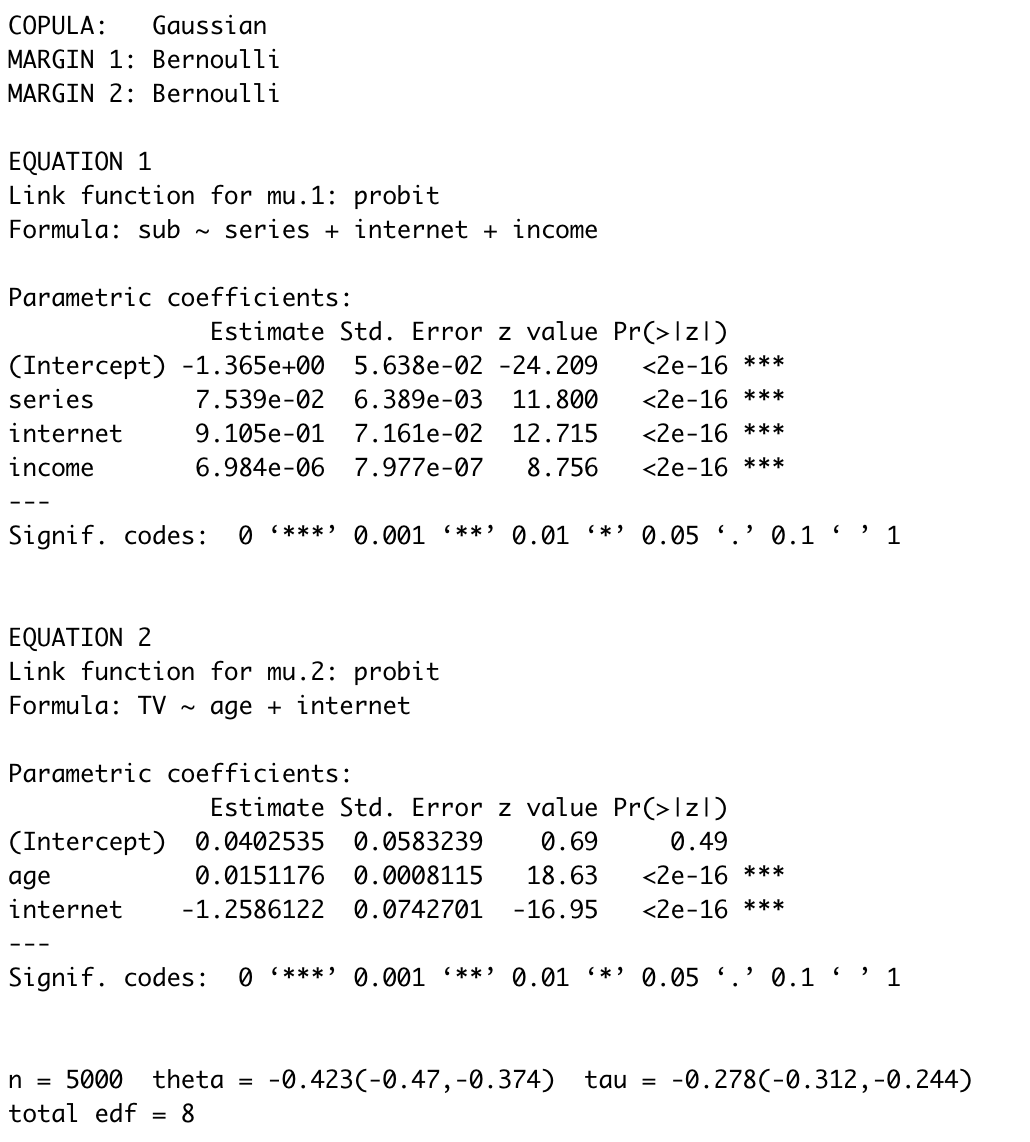
\includegraphics[scale=0.6]{system1.png}
	\end{figure}

		\subsection{Задание №6.2.}
		\textit{
	Проинтерпретируйте оценки коэффициентов при независимых переменных и коэффициента корреляции между случайными ошибками рассматриваемых уравнений.}

	\vspace{0.2cm}
	
	Оценка ковариационной матрицы для нормально распределенных случайных ошибок модели имеет следующий вид:
	\[
	\widehat{\Sigma} = 
	\begin{bmatrix}
		1 & -0.4227924 \\
		-0.4227924 & 1 
	\end{bmatrix}
	\]
	
	То есть коэффициент корреляции между случайными ошибками в двух уравнениях отрицателен. Следовательно, как и было описано в предположениях, может иметь место взаимозаменяемость подписки на онлайн кинотеатр телевидения: наличие подписки снижает вероятность просмотра телевизора, а частый просмотр ТВ уменьшает вероятность наличия подписки на онлайн кинотеатр.
	
	Интерпретируя оценки коэффициентов видно, что все выбранные коэффициенты значимы в том направлении, в котором предполагалось (кроме общей независимой переменной). То есть доход и количество просмотренных сериалов положительно влияют на вероятность наличия подписки, а для вероятности частого просмотра телевидения видно, что чем старше индивид, тем вероятнее он чаще смотрит телевидение. Для того чтобы оценить влияние доля времени в интернете нужно оценивать предельные эффекты, что будет сделано далее.

		\subsection{Задание №6.3.}
		\textit{
	При помощи LR теста проверьте, имеется ли необходимость в том, чтобы оценивать оба уравнения совместно.
				}
			
			\vspace{0.2cm}
			
			Нулевая гипотеза будет заключаться в том, что корреляция равна 0.
			
			\begin{equation*}
				\begin{cases}
					H_0: \rho = 0\\
					H_a: \rho \ne 0
				\end{cases}
			\end{equation*}
			
			Статистика теста $LR= 2(\ell_{UR} - \ell_{R})$ распределена как хи-квадрат с 1 степенью свободы (одно ограничение на параметр модели). 
			
			Проведя тест найденное p-value равно 2.146829e-52, то есть нулевая гипотеза отвергается, а значит, уравнения необходимо оценивать совместно.
	
		\subsection{Задание №6.4.}
		\textit{
	Для индивида с произвольными характеристиками оцените:
	\begin{enumerate}
		\item Вероятность подписки
		\item Вероятность того, что индивид смотрит телевизор по крайней мере раз в неделю
		\item Вероятность того, что индивид и имеет подписку, и смотрит телевизор не реже раза в неделю
		\item Вероятность того, что у индивида имеется подписка, при условии, что он смотрит телевизор реже раза в неделю
	\end{enumerate} }

	\vspace{0.2cm}
	
	Возьмем индивида с такими характеристиками, представленные в Таблице \ref{individ2}:
	
\begin{table}[!h]
	\caption{Характеристики рассматриваемого индивида в системах уравнений}
	\label{individ2}
	\centering
	\small
	\begin{tabular}{|c|c|}
		\hline
		Переменная &  Значение  \\ 
		\hline
		$series_{ind} $ &4 \\ 
		\hline
		$internet_{ind} $ &0.7 \\ 		
		\hline
		$income_{ind} $ &50000 \\ 	
		\hline
		$age_{ind} $ &21 \\ 
		\hline
	\end{tabular}
\end{table}

	Посчитаем вероятности для каждого пункта отдельно:

	\begin{enumerate}
		\item $\widehat{P} (sub_{ind}=1)=  \mathcal{F} (\hat{\beta_0} + \hat{\beta_1}\times series_{ind}+ \hat{\beta_2} \times internet_{ind} +\hat{\beta_3}\times income_{ind}) = 0.4693562$
		
		То есть у индивида вероятность наличия подписки без учета второго уравнения и частоты просмотра ТВ равна примерно 46\%.
		
		\item $\widehat{P} (TV_{ind}=1)= \mathcal{F} (\hat\gamma_0 + \hat\gamma_1 internet_{ind}+ \hat\gamma_2 age_{ind}) = 0.3003812$
		
		То есть у индивида вероятность частого просмотра телевидения без учета первого уравнения и наличия подписки на онлайн кинотеатр равна примерно 30\%.
		
		\item $\widehat{P} (sub_{ind}=1, \, TV_{ind}=1) = \mathcal{F} (\widehat{sub_{ind}^*}, \widehat{TV_{ind}^*}; , \hat\rho) = 0.04156213$
	
		Где $\widehat{sub_{ind}^*}, \widehat{TV_{ind}}^*$ - оцененные вероятности для индивида в двух уравнениях, а $\mathcal{F} $- двумерное нормальное распределение.
		
		То есть у индивида вероятность частого просмотра телевидения и наличия подписки на онлайн кинотеатр равна примерно 4\%.
			
		\item $\widehat{P} (sub_{ind}=1 \,|\, TV_{ind}=0) = \dfrac{\widehat{P} (sub_{ind}=1, TV_{ind}=0)}{\widehat{P} (TV_{ind}=0)} = \dfrac{\widehat{P}(sub_{ind}=1, TV_{ind}=0)}{1-\widehat{P} (TV_{ind}=1)} = 0.369943$
		
		То есть у индивида вероятность наличия подписки на онлайн кинотеатра при условии, что он не часто смотрит телевидение равна примерно 37\%.
		
	\end{enumerate}

	\newpage
	\section{Часть 7. Сравнение моделей}
	
	\subsection{Задание №7.1.}
	\textit{
	Определите, какая из оцененных вами моделей обладает наибольшей предсказательной силой. }
	
	\vspace{0.2cm}
	
	Ниже представлена Таблица \ref{accuracymodels} для сравнения прогностических сил ($accuracy$)моделей.
	
		\begin{table}[!h]
		\caption{Доли верных предсказаний пробит, линейной-вероятностной, наивной модели, логит модели и модели системы бинарных уравнений}
		\label{accuracymodels}
		\centering
		\begin{tabular}{|c|c|}
			\hline
			Модель  &  Доля верных предсказаний  \\ 
			\hline
			Пробит модель& 0.6760\\
			\hline
			Наивная модель & 0.6446\\
			\hline
			Линейно-вероятностная модель &0.6774	\\		
			\hline
			Логит модель&0.6754	\\	
			\hline
			Система бинарных уравнений&0.6466	\\	
			\hline
		\end{tabular}
	\end{table}

	Можно сказать, что предсказательная сила пробит и логит моделей лучше наивной модели, но хуже чем у линейной-вероятностной модели. А модель с системой бинарных уравнений и вовсе не сильно лучше наивной модели, что может быть вызвано другой функциональной формой и не учетом важных факторов (как возраст в квадрате). 
	
	Таким образом, по предсказательной силе наилучшая модель - линейно-вероятностная модель, хотя как уже было выше отмечено, она трудноинтерпретируема и имеет ряд недостатков.

	
		\subsection{Задание №7.2.}
		\textit{
	Выберите лучшую из оцененных вами моделей руководствуясь информационными критериями. }

	\vspace{0.2cm}
	
	Ниже представлена Таблица \ref{aicmodels} для сравнения моделей по информационным критерям AIC, BIC, которые считаются по следующим формулам:
	\begin{align*}
		& \text{AIC} = 2k - 2\ln (\hat L) \\
		& \text{BIC} = k \ln (n) - 2\ln (\hat L)
	\end{align*}

	Как видно из Таблицы \ref{aicmodels}, логит и пробит модели лучшие модели с наименьшими показателями по AIC, BIC и практически одинаковы с небольшим перевесом у логит модели. При этом линейно-вероятностная модель хоть и хуже этих моделей (показатели критериев выше), но модель с системой бинарных уравнений намного хуже. Это вызвано тем, что она оценивает сразу два уравнения, поэтому для сравнения нужно и по другим моделям оценить 2 уравнения. 
	
	\begin{table}[!h]
		\caption{Общие информационные критерии AIC, BIC для пробит, линейной-вероятностной, наивной модели, логит модели и модели системы бинарных уравнений}
		\label{aicmodels}
		\centering
		\begin{tabular}{|c|c|c|}
			\hline
			Модель  &  AIC&BIC  \\ 
			\hline
			Пробит модель& 6057.949&6103.570\\
			\hline
			Линейно-вероятностная модель &6365.681&6417.819\\		
			\hline
			Логит модель&6057.887&6103.507\\	
			\hline
			Система бинарных уравнений&11954.374&12006.511\\	
			\hline
		\end{tabular}
	\end{table}

	В таблице \ref{aicbicmodels} представлены результаты после оценивания 2 уравнений каждой из модели и сложением AIC и BIC по двум уравнениям для всех моделей, кроме системы. 
	
	\begin{table}[!h]
		\caption{Информационные критерии AIC, BIC для пробит, линейной-вероятностной, наивной модели, логит модели и модели системы бинарных уравнений для 2 выбранных уравнений}
		\label{aicbicmodels}
		\centering
		\begin{tabular}{|c|c|c|}
			\hline
			Модель  &  AIC&BIC  \\ 
			\hline
			Пробит модель& 12238.62&12284.24\\
			\hline
			Линейно-вероятностная модель &12868.13&12926.79\\		
			\hline
			Логит модель&12242.08&12287.70\\	
			\hline
			Система бинарных уравнений&11954.374&12006.511\\	
			\hline
		\end{tabular}
	\end{table}
	
	Можно отметить, что в этом случае логит и пробит модель также близки по информационным критериям с небольшим улучшением у пробит модели в этот раз. Они также  лучше линейно-вероятностной, хотя были хуже ее по прогностической силе. Однако модель с системой бинарных уравнений является лучше других моделей (критерии AIC, BIC меньше всего), что объясняется тем, что уравнения необходимо оценивать вместе (даже специально проверяли гипотезу на совместимость оценивания уравнений).
	
	То есть лучшая модель по информационным критериям - модель с системой бинарных уравнений.

	\newpage

	\section{Часть 8. Модель бинарного выбора со случайными ошибками, имеющими распределение Стьюдента}
	
	Число степеней свободы в данном задании будет равно $df = 13$.
	
	\subsection{Задание №8.1.***}
	\textit{
	Используя воображение придумайте и кратко опишите экономическую задачу, для решения которой необходимо применить модель бинарного выбора. Например, можно рассмотреть влияние различных факторов на вероятность дефолта банка. Укажите зависимую переменную и по крайней мере три независимых, а также кратко опишите предполагаемый механизм влияния независимых переменных на зависимую. 
	}

	\vspace{0.2cm}

	Будем рассматривать задачу по определению факторов, влияющих на частое употребление кофе. Это достаточно важная задача особенно для компаний-производителей и самих продавцов кофе, ведь им важно узнать останется ли с ними человек и продолжит часто покупать и пить кофе.
	
	То есть в качестве зависимой переменной будет выступать $coffee$ - дамми переменная на то, что человек пил кофе за последнюю неделю.
	
	В качестве независимых переменных рассмотрим такие факторы, влияющие на употребление кофе:
	
	\begin{itemize}
		\item $income$  - Доход индивида 
		
		Он влияет на факт употребления кофе, так как кофе является не таким дешевым продуктом и многие просто могут себе не позволить покупать его. Поэтому ожидается, что больше и чаще пьют кофе более люди с более высоким заработком. Учитывая лог-нормальность распределения, то в моделях доход будет рассматривается с использованием логарифмирования.
		
		Гипотеза: доход положительно влияет на частоту употребления кофе.
		
		\item $age$  - Возраст индивида 
		
		Явно влияет на факт употребления кофе, так как чаще пьют кофе те, кто хочет не уснуть и к таким больше относятся молодые люди (студенты) и зрелые (рабочие люди). А более пожилые люди заинтересованы заботой своим здоровьем и будут реже пить кофе.
		
		Гипотеза: возраст отрицательно влияет на частоту употребления кофе.
		
		\item $cigarette$ - Дамми переменная для курящих людей
		
		Выбрана эта дамми, так как если человек имеет одну зависимость в форме никотина, то скорей всего, будет склонен и к другим зависимостям.
		
		Гипотеза: факт курения положительно влияет на частоту употребления кофе.
		
	\end{itemize}
	
	\subsection{Задание №8.2.***}
	\textit{
	Симулируйте процесс генерации данных, соответствующий вашей задаче в логике бинарной модели со случайными ошибками, имеющими распределение Стьюдента (по аналогии с тем, как это делалось для обычной пробит модели для дефолта на семинаре). В тексте работы этот пункт отражать не нужно, достаточно реализовать его в коде. Все дальнейшие пункты выполняются на симулированных данных из выборки объемом 5000 наблюдений. Перед началом симуляций необходимо указать set.seed(123). 
}

	\vspace{0.2cm}
	
	Модель и истинные значения коэффициентов предположим такими (всего будет 60\% любителей кофе в выборке):
	
	\begin{align*}
		P(coffee=1) = 1+0.5\times log(income)-0.09\times age+0.2\times cigarette
	\end{align*}
	
	\subsection{Задание №8.3.***}
	\textit{
	Оцените параметры вашей модели с использованием бинарной модели со случайными ошибками, имеющими распределение Стьюдента с 13 степенями свободы. Результат представьте в форме таблицы, содержащей оценки коэффициентов и p-value тестов на значимость.
}

\vspace{0.2cm}

Полученные результаты представлены в Таблице \ref{mymodel}. Как легко заметить, полученные коэффициенты достаточно близки к истинным значениям и значимы, а также подтверждают вынесенные выше гипотезы.

\begin{table}[!h]
	\caption{Оценки бинарной модели со случайными ошибками, имеющими распределение Стьюдента с 13 степенями свободы}
	\label{mymodel}
	\centering
	\begin{tabular}{|c|c|c|}
		\hline
		Переменная  &  $\hat{\beta}$& p-value  \\ 
		\hline
		Constant & 0.43759880&3.249177e-01\\
		\hline
		log(income)&0.60110278***&0.000000e+00\\		
		\hline
		age&-0.09669452***&1.585945e-279\\	
		\hline
		cigarette&0.17861389***&4.985862e-03\\	
		\hline
	\end{tabular}
\end{table}
	          
	
\end{document}